\chapter{Evaluation}
\label{cha:evaluation}

In this chapter, we present the first set of results and insights drawn from our NTT architecture. We begin with an overview of the data and setup for evaluation, followed by an initial evaluation and use the results from this,  to draw further insights and carry out further, more robust evaluation.

\section{Initial Evaluation Setup}
\label{eval:evaldat}

We have already discussed in detail the dataset used for pre-training in Section \ref{sec:ns3} and the objectives in Section \ref{ssec:despatt}. For testing the initial performance of our pre-training process, we reserve a random $10\%$ of the sequences from our pre-training data. This data is always used just for testing and the model does not see this data during the pre-training phase ever. 

\begin{figure}[h]
  \begin{center}
    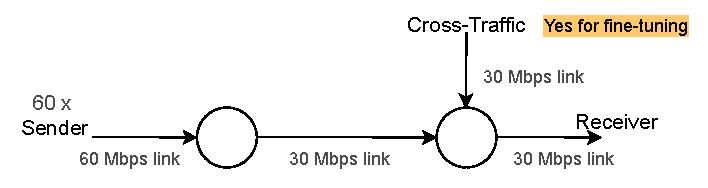
\includegraphics[scale=1.2]{figures/simple_topo_ft.pdf}
    \caption{Fine-tuning data generation}
    \label{fig:topo_ft}
  \end{center}
\end{figure}

The setup for the fine-tuning dataset is the same, except that we add a second bottleneck for sender traffic by introducing $20$ Mbps of TCP cross-traffic on the rightmost link. The dataset does \emph{not} explicitly contain the cross-traffic; we \emph{only} collect packets from the senders. However, the introduction of this cross traffic affects the dynamics of the overall network due to  congestion, which in turn affects the dynamics in the behaviour of the applications sending traffic. We demonstrate this setup in Figure \ref{fig:topo_ft}. For our initial evaluation, we generate one simulation run of fine-tuning data only and this dataset contains about 115 thousand packets, \ie roughly $1/10$\textsuperscript{th} of the pre-training dataset. To ensure our training is not affected by extremely large possible ranges of values, we normalise our input features of size and delay, over the mean and standard deviation of each feature over the entire data, individually.\cite{scaling} Based on the fine-tuning dataset generated, we have two fine-tuning tasks 

\begin{itemize}
\item \emph{Fine-tuning on new environment:} In this fine-tuning task, we try to predict the last delay in the sequence, on data generated on a new topology with $2$ bottlenecks, as opposed to pre-training where we had $1$ bottleneck. Our pre-training process employs multiple kinds of masking over different delay positions, but for the fine-tuning task objective is prediction of the delay at the last position. The \emph{key idea} is to use the learn sequence structure in the during the pre-training and apply it to predict the last delay and make a decision on the final packet during the fine-tuning, following a change in network environment. We expect that if the pre-training is done robustly, fine-tuning in this new environment on a similar task will be both faster and require significantly less data.

\item \emph{Fine-tuning on a new task:} In this fine-tuning task, we try to predict the Message Completion Time (MCT) of an entire transmitted message, given the NTT's encoded output states of the previous $1024$ packets and the size of the given message. Our fine-tuning objective is to mean pool\cite{poolcv}\cite{zaheerDeepSets2018} over all the NTT's output states which represents the overall learnt behaviour of the network dynamics in the recent past. We combine this learnt feature with the message size, which we can have in our simulation data using appropriate features from our Network Simulator\cite{ns3} and use this to predict the MCT using a Multilayer Perceptron with linear layers. The \emph{key idea} is to learn the \emph{overall} structure from the network dynamics and use it to predict tasks, which depend on the nature of these dynamics.
\end{itemize}

We report the mean-squared error (MSE) for achieved on both tasks and report our initial findings in Table \ref{eval:table1}.
We process MCTs on a logarithmic scale to limit the impact of outliers. This is required as our MCT dataset is quite heavy tailed, which hurts training deep learning models.\footnote{Our simulation's mean and 99.9th percentile MCTs are 0.2 and 23 seconds, respectively.}


\section{Preliminary Results}
\label{eval:pres}

In our initial experiments, we compare several versions of our NTT, vary both our pre-training and fine-tuning objectives, in order to explore the possibilities of what information can actually be learnt and to which extent. We focus on evaluating and demonstrating on the following points:

\begin{itemize}
\item Our NTT is capable of learning network dynamics from packet data 
\item Pre-training enables our NTT to generalize on new environments and new tasks 
\item Incorporating our networking domain specific knowledge helps the NTT perform better
\end{itemize}

We demonstrate our initial comparison in Table \ref{eval:table1} The \emph{pre-trained} model first learns from the pre-training and then from the fine-tuning dataset, while the \emph{from scratch} version only learns from the fine-tuning dataset. In these experiments, the fine-tuning dataset is only around $1/10$\textsuperscript{th} of the size of the pre-training dataset. In all the NTT variants presented here, we only mask the last packet delay during the pre-training process.

In order to evaluate the choice of our feature selection for pre-training , we perform some ablation studies on the input data. We argue that we need both packet state information and network state information to effectively learn network dynamics. In order to investigate this, we pre-train two additional versions of the NTT, one \emph{without delay} and one \emph{without packet size} information, in the respective input sequences.

We also perform ablation studies to investigate the effects of aggregating features in our input, which we feed into the encoder stage of our NTT. Concretely, we compare our multi-step aggregation of $1024$ packets into $48$ aggregates (see Section \ref{ssec:desagg}) with \emph{no aggregation} (using only $48$ individual packets) and \emph{fixed aggregation} (using $48 $aggregates of $21$ packets each, \ie $1008$ packet sequences). Due to limits of our training infrastructure and Transformer's quadratic scaling behaviour with increasing sequence size, it is infeasible to evaluate the effects of having no aggregation on very large sequences.



\begin{table}[htbp]
\centering
\begin{tabular}{ l   c   c  c }
\toprule
\emph{all values $\times10^{-3}$} & Pre-training  & \multicolumn{2}{c}{Fine-tuning} \\
\cmidrule{3-4}
                                                       & {Delay}        & {Delay}                           & {log MCT} \\
\midrule
\em{NTT}                                                 &                &                                   &           \\
    \smallindent Pre-trained                                 & 0.072          & 0.097                             & 65        \\
    \smallindent From scratch                                & {-}            & 0.313                             & 117       \\
    \noalign{\vskip 1mm}
    \em{Baselines}                                                                                                                 \\
    \smallindent ARMA                                            & 1.800        &  1.180                              &1412 \\
    \smallindent Last observed                               & 0.142          & 0.121                             & 2189      \\
    \smallindent EWMA                                        & 0.259          & 0.211                             & 1147      \\
    \noalign{\vskip 1mm}
    \em{NTT (Ablated)}                                                                                                        \\
    \smallindent No aggregation                              & 0.258          & 0.430                             & 61        \\
    \smallindent Fixed aggregation                           & 0.055          & 0.134                             & 115       \\[0.75mm]

    \smallindent Without packet size                         & 0.001          & 8.688                             & 94        \\
    \smallindent Without delay                               & 15.797         & 10.898                            & 802       \\
     \bottomrule

\end{tabular}
\caption{Mean Squared Error for all initial NTT models and tasks.}
\label{eval:table1}
\end{table}

We also to ensure that we understand if our NTT learns useful information in the first place. To put this into perspective, we use the following three simple baselines in order to compare the performance of our different NTT variants. 
\begin{itemize}
\item \emph{Auto-Regressive Moving Average (ARMA):} In this method, we predict the mean delay of all the previous delay values in our sequence as our target delay value.
\item \emph{Last observed:} In this method, we predict the last observed delay over all the previous delay values in our sequence as our target delay value.
\item \emph{Exponentially Weighted Moving Average (EWMA):}  In this method, we predict a weighted smoothed mean delay of all the previous delay values in our sequence as our target delay value.\footnote{For our EWMA, we use the decay factor $\alpha=0.01$} 
\end{itemize}

\paragraph*{NTT can learn some network dynamics:}

Based on the initial evaluation, we confirm that the \emph{pre-trained} NTT beats our baselines in all cases. Though the baselines are rather basic, we can already conclude that the NTT learns the network dynamics to an extent and that the 
the error values are sensible. We also observe that some of the baselines work reasonably, depending on the complexity of the task. For \eg the smoothed \emph{EWMA} approach works reasonably well for delay prediction, it fails for the more complex MCT task.
On the delay task, we further observe that the \emph{last observed} baseline performs better than \emph{EWMA}; that is, smoothing over a long sequence performs worse than simply returning the most recent packet.
This suggests that there is something to learn from the \emph{sequence dynamics}, which the NTT can do much better, as we see it perform better for both types of fine-tuning tasks. This suggests that the NTT can learn fine-grained sequence information, along with aggregated structural information from the entire sequence.

\begin{figure*}[!h]
  \begin{center}
    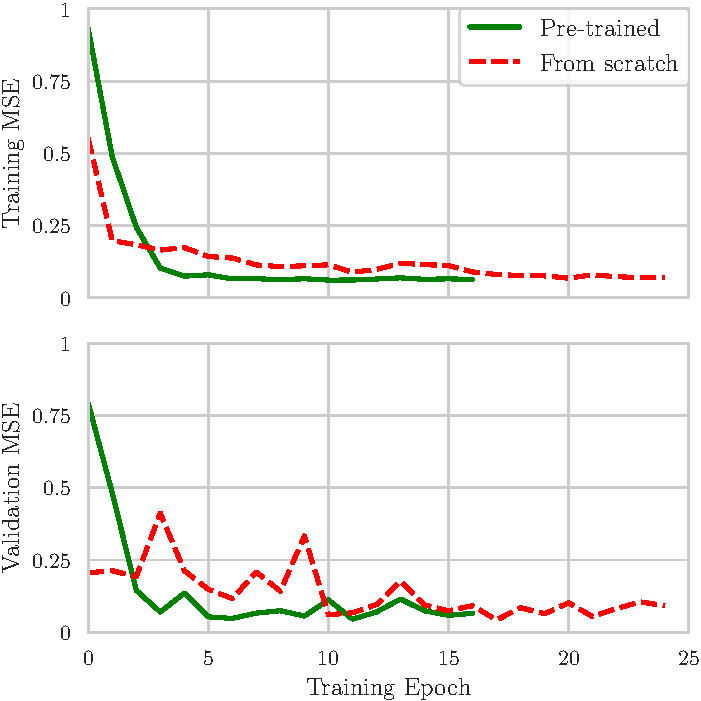
\includegraphics[scale=1]{figures/MCT_loss.pdf}
    \caption{Mean-square error for prediction of message
time completion over training epochs}
    \label{fig:loss_mct}
  \end{center}
\end{figure*}

\vspace{-1cm}

\paragraph*{NTT can generalize across environments and tasks:}

We observe that pre-training is beneficial: on both fine-tuning tasks, the \emph{pre-trained} NTT outperforms the \emph{from scratch} version.The pre-training knowledge generalizes to a new environment \ie unobserved cross-traffic and to a new task \ie MCT prediction. In our current NTT variants, we pre-train and fine-tuning for delay prediction in the exact same way, by learning to predict the last delay in the sequence. Pre-training also improves the speed of the fine-tuning process, in addition to the overall performance. We see this in Figure \ref{fig:loss_mct} shows that pre-training allows faster learning on the fine-tuning dataset: the \emph{pre-trained} NTT reaches a lower error after a few (only 3) training epochs and finishes training, \ie no further improvement, after fewer epochs (16 vs 24), with a lower MSE on the test set in the end (Table \ref{eval:table1})


\paragraph*{NTT specific features help:}
Finally, we observe the benefits of the two NTT-specific features we propose: \ie the hierarchical aggregation layer and the mix of network and traffic information in the raw data.

With \emph{no aggregation}, the model has little history available; we observe that, perhaps surprisingly, this affects the delay predictions, but not the MCT ones. Conversely, with a \emph{fixed aggregation}, the model loses recent packet-level details but has access to longer history; this seems sufficient to predict delays but affects the MCT.\footnote{In the vision transformer\cite{dosovitskiyImageWorth16x162021}, they got extremely good results with fixed size aggregations and very large training datasets.}
It is a little early to map the exactness of these effects at this point, however we can conclude from this initial result suggests that both recent packet level information and longer historical aggregates are useful to generalize to a large set of tasks.


Considering the NTT versions \emph{without packet size} and \emph{without delay} information (Table \ref{eval:table1}), we observe that neither generalize well.
Without the packet size, the model overfits the pre-training dataset and performs poorly on predicting delay for fine-tuning.
Without delay information, the model can logically not produce any useful prediction related to packet delays or MCTs.


Based on the promising nature of our initial results, we now move to more robust evaluation, harder and more generic pre-training and fine-tuning objectives, in order to explore to what further extent can our NTT perform. We explore further methods to improve our NTT in the following Section \ref{eval:fres}


\section{Further Results}
\label{eval:fres}

\subsection{NTT vs improved baselines}
\label{ssec:impbase}

\begin{itemize}
\item ARIMA (both 10000 and 30000 history)
\item Bi-LSTM (all studies)
\end{itemize}

\subsection{Robust fine-tuning evaluation}
\label{ssec:robeval}

\begin{itemize}
\item pre-train + fine-tune on $10 \%$  
\item pre-train + fine-tune on  $100 \%$  
\item from scratch + fine-tune on $10 \%$  
\item from scratch + fine-tune on $100 \%$  
\end{itemize}

\subsection{Improved pre-training for NTT}
\label{ssec:impptt}

\begin{itemize}
\item variable masking, last 16
\item variable masking, last 32
\item mask over non-aggregate + aggregate, uniform choice over states
\item mask over non-aggregate + aggregate, uniform choice over aggregation level 
\item multi instances of decoders 
\end{itemize}

\subsection{Evaluation on complex topologies}
\label{ssec:comptop}



